\subsection{Dallamszerkesztés példa}
\begin{pitemize}
Funkció & T & ST(SD) & M(D,T) & SD & D & SM(SD,T) & V(D) \\ \hline
Az skála hangjai & A & H & \cisz & D & E & \fisz & \gisz \\
Hármashangzatai & $A$ & $H_m$ & $C^\#_m$ & $D$ & $E$ & $F^\#_m$ & $G^{\#\dim}$ \\
Négyeshangzatai & $A^{maj7}$ & $H_m^7$ & $C^{\#7}_m$ & $D^{maj7}$ & $E^{7}$ & $F^{\#7}_m$ & $G^{\#\sdim7}$ \\ 
Ötöshangzatai & $A^{maj9}$ & $H_m^9$ & $C^{\#9b}_m$ & $D^{maj9}$ & $E^{9}$ & $F^{\#9}_m$ & $G^{\#\sdim9b}$
\end{pitemize}
Horizontális felfogásban a skála akkordjait a skála hangjaiból álló dallam kíséri.
Hogy egy kicsit érdekesebben hangozzék, két ütemen keresztül a funkciót vertikálisan értelmezzük.
A következő lépés azon skálák meghatározása, melyekben az általunk kiválasztott kísérő akkordok szerepelnek. Ezúttal legyen ez a domináns $E^7$.
Vizsgáljunk meg pár szóbajöhető skálatípust! 
Vizsgáljuk meg a hangközöket és a fokokról induló hangzatok típusait: \\
\begin{minipage}[t]{0.5\textwidth}
\begin{flushleft}
\begin{pitemize}
\multicolumn{4}{c}{melodikus moll} \\ \hline
fok   & hangköz   & hármas & négyes & ötös \\ \hline
I     & p   & dúr  & mollmaj7  & mollmaj9 \\
II    & n2  & moll & moll7     & moll9b \\
III   & k3  & moll & bővmaj7   & bővmaj9 \\
IV    & t4  & dúr  & \bf{dom7} & dom9 \\
V     & t5  & dúr  & \bf{dom7} & dom9b \\
VI    & k6  & moll & félszűk7  & félszűk9 \\
VII   & n7  & szűk & félszűk7  & félszűk9b \\
\end{pitemize}
\end{flushleft}
\end{minipage}
\begin{minipage}[t]{0.45\textwidth}
\begin{flushright}
\begin{pitemize}
\multicolumn{4}{c}{harmonikus moll} \\ \hline
fok   & hangköz   & hármas & négyes & ötös \\ \hline
I     & p   & moll & mollmaj7  & mollmaj9 \\
II    & n2  & szűk & félszűk7  & félszűk9b \\
III   & k3  & bőv  & bővmaj7   & bőv9 \\
IV    & t4  & moll & moll7     & moll9 \\
V     & t5  & dúr  & \bf{dom7} & dom9 \\
VI    & n6  & dúr  & maj7      & maj9 \\
VII   & n7  & szűk & szűk7     & szűk9b \\
\end{pitemize}
\end{flushright}
\end{minipage}
\\\\
A melodikus moll skála negyedik fokán, a kulcshangtól kvart távolságra elhelyezkedő 
$E^{7}$-hez a hangközfordítás szabályai szerint a kulcshang E-től tiszta kvint távolságra van,
tehát a keresett skála az $H_m$: \\
H, \cisz, D, E, \fisz, \gisz, \aisz. \\\\
A melodikus moll skála ötödik fokán, a kulcshangtól kvint távolságra elhelyezkedő 
$E^{7}$-hez a hangközfordítás szabályai szerint a kulcshang E-től tiszta kvart távolságra van,
tehát a keresett skála az $A_m$: \\
A, H, C, D, E, \fisz, \gisz. \\\\
A harmonikus moll skála ötödik fokán, a kulcshangtól kvint távolságra elhelyezkedő 
$E^{7}$-hez a hangközfordítás szabályai szerint a kulcshang E-től tiszta kvart távolságra van,
tehát a keresett skála az $A_m$: \\
A, H, C, D, E, F, \gisz. \\\\
Az utolsó kettőből és az alapskálából alkotott kilenc fokú alterált skála: \\
A, H, C, \cisz, D, E, F, \fisz, \gisz \\\\
Pillér hangok $E^7$-hez: \\
E, \gisz, H, D \\\\
Diatonikus váltóhangok (az A dúr skála A, H, \cisz, D, E, \fisz, \gisz hangjait elhagyva): \\
C, F \\\\
Kromatikus váltóhangok: \\
E pillérhanghoz: \disz \\
\gisz pillérhanghoz: G, \aisz \\
H pillérhanghoz: \aisz \\
D pillérhanghoz: \disz \\

Az első öt ütem horizontális értelmezés szerint a skála hangjaival kísért akkordokat tartalmaz.
A következő kettő érdekesebben hangzik: a dallammenet  E - \aisz - H - D, \gisz - D - H - \gisz. Az első -és harmadik negyed pillér hang. A H hangot a kromatikus váltóhangja, \aisz előzi meg.

\begin{figure}[!htbp]
 \advance\leftskip-6mm
 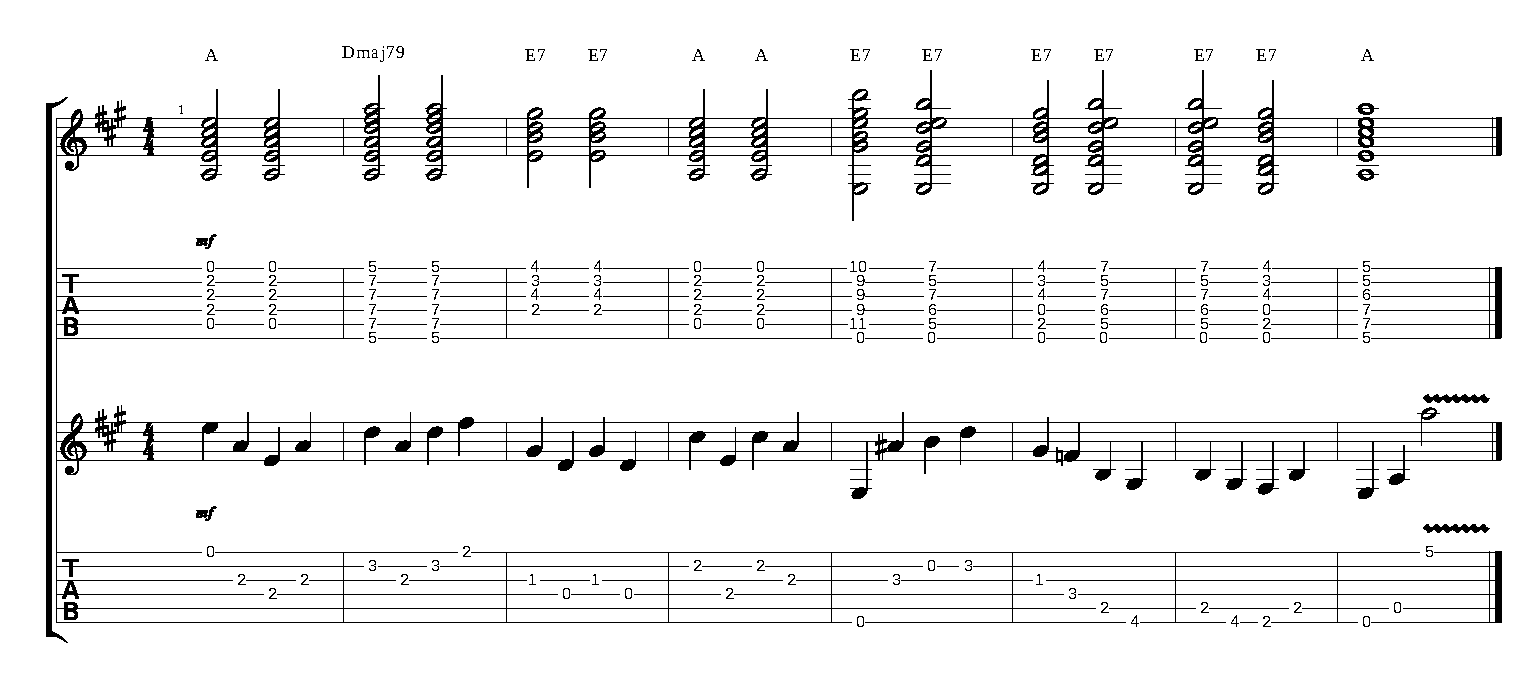
\includegraphics[page=1,scale=0.70]{kottak/dallamszerkesztes.pdf}
\end{figure}
